\documentclass{article}
\usepackage[utf8]{inputenc}
\usepackage{tikz}
\usetikzlibrary{external}
\tikzexternalize
\begin{document}

%4 5
%10 20
%11 15
%9 30
%32 11

%15 14
%29 11
%9 26
%9 30
%1 1

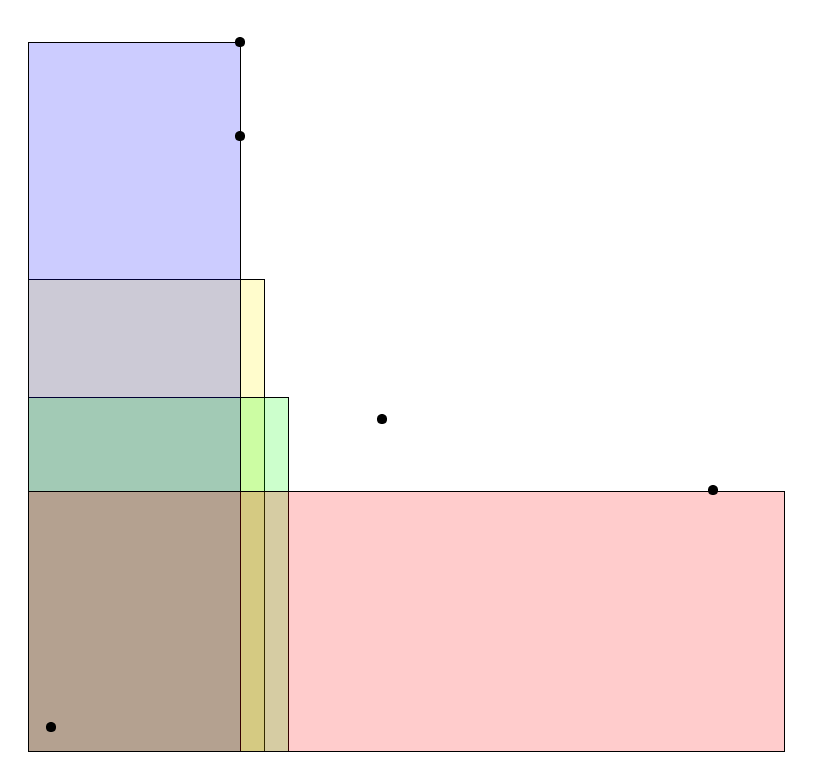
\begin{tikzpicture}[scale=0.3]

\draw[fill=yellow, fill opacity=0.2] (0, 0) rectangle (10, 20);
\draw[fill=green, fill opacity=0.2] (0, 0) rectangle (11, 15);
\draw[fill=blue, fill opacity=0.2] (0, 0) rectangle (9, 30);
\draw[fill=red, fill opacity=0.2] (0, 0) rectangle (32, 11);

\foreach \Point in {(15, 14), (29, 11), (9, 26), (9, 30), (1, 1)}{
    \node at \Point {\textbullet};
}


\end{tikzpicture}

\end{document}

